\section{Χαρακτηριστικά εκδόσεων \en{OpenMP} 3.0 - 4.5}
\subparagraph{}
To \en{OpenMP} 3.0 ήταν η πρώτη ενημέρωση μετά την έκδοση 2.5 με σημαντικές προσθήκες και αλλαγές. Χαρακτηριστικά προηγούμενων εκδόσεων αναβαθμίστηκαν αλλά τη σημαντικότερη αλλαγή αποτέλεσε η εισαγωγή στην έννοια των διεργασιών (\emph{\en{Tasking}}). Η επόμενη έκδοση του \en{OpenMP} (4.0) κυκλοφόρησε τον Ιούλιο του 2013 και περιελάμβανε τα παρακάτω χαρακτηριστικά:
\begin{itemize}
    \item \en{threads affinity},
    \item ετερογενείς προγραμματισμός,
    \item διαχείριση σφαλμάτων,
    \item διανυσματικοποίηση μέσω \emph{\en{SIMD}},
    \item \emph{\en{user-defined recuctions (UDRs)}}

\end{itemize}


Το 2013 με την έκδοση 4.0, οι προδιαγραφές του OpenMP έκαναν σημαντικές αλλαγές στην υποστήριξη για ετερογενών συστημάτων. Εισήχθει ένα σύνολο οδηγιών για τον προσδιορισμό συναρτήσεων και δεδομένων που θα μετακινηθούν σε συσκευή προορισμού για να υπολογιστούν. Εκτός όμως απο των υποστήριξη επιταχυντών, εισήχθει και η \emph{\en{SIMD}} υποστήριξη για διανύσματα, ο \emph{\en{thread affinity}} έλεγχος, τα \emph{\en{user-defined reductions (UDRs)}}, η δημιουργία διεργασιών και φράσεις εξάρτησης. 
Η κυκλοφορία της έκδοσης 4.5 έγινε το 2015, και περιείχε την \emph{\en{taskloop}} οδηγία που θα επέτρεπε τον διαχωρισμό των βρόγχων σε διεργασίες, αποτρέποντας όλα τα νήματα να εκτελέσουν τον βρόγχο.

Τέλος, παρείχθει υποστήριξη για βρόχους \emph{\en{doacross}} να παραλληλίσουν τους βρόχους με καλά δομημένες εξαρτήσεις και εισήχθη περαιτέρω υποστήριξη για διεργασίες με τη μορφή προτεραιότητας διεργασιών.
Επεκτάσεις στο \emph{\en{SIMD}} περιελάμβαναν τη δυνατότητα καθορισμού ακριβούς πλάτους \emph{\en{SIMD}} και επιπλέον
χαρακτηριστικών κοινής χρήσης δεδομένων\cite{pros2}.
\clearpage

\subsection{\en{SIMD}}
\subparagraph{}

\textbf{ΝΑ ΔΩ ΤΟ ΚΡΙΣΤΥ ΓΟΥΝΤΣ ΒΕΚΤΟΡΙΖΑΤΙΟΝ!}
Σύμφωνα με τον \emph{\en{Flynn}} \cite{flynn}, ένας επεξεργαστής \emph{\en{Single Instruction Multiple Data (SIMD)}} δημιουργεί παραλληλισμό δεδομένων παρέχοντας οδηγίες που λειτουργούν συνολικά σε μπλοκ δεδομένων που ονομάζονται διανύσματα. Αυτό έρχεται σε αντίθεση με τις βαθμωτές οδηγίες που εκτελούνται σε μοναδιαία στοιχεία κάθε φορά.

Στο \emph{\en{OpenMP}}, διανυσματικοποίηση αναφέρεται ως ο παραλληλισμός \emph{\en{SIMD}}. Το \emph{\en{SIMD}} παρέχει παραλληλισμό δεδομένων σε επίπεδο εντολών, δηλαδή μια οδηγία λειτουργεί ταυτόχρονα με πολλά στοιχεία δεδομένων. Οι \emph{\en{SIMD}} οδηγίες χρησιμοποιούν ειδικούς καταχωρητές που περιέχουν πολλαπλά δεδομένα. Το μέγεθος αυτών των καταχωρητών ορίζει το μήκος του διανύσματος που είναι ο αριθμός των βαθμωτών δεδομένων που μπορούν να υποστούν επεξεργασία παράλληλα σε μια οδηγία \emph{\en{SIMD}}.

Στο παρακάτω σχήμα παρουσιάζεται η προσθεση των στοιχείων δυο διανυσμάτων και η εκχώρηση των αποτελεσμάτων σε ένα τρίτο, με τον συμβατικό τρόπο, αλλά και με την χρήση \emph{\en{SIMD}} μεθόδου. Το πλεονέκτημα είναι οτι οι \emph{\en{SIMD}} οδηγίες εκτελούνται το ίδιο γρήγορα με τις αντίστοιχες βαθμωτές. Με άλλα λόγια η πράξη της παρακάτω εικόνας, θα γίνει 4 φορές που γρήγορα αν χρησιμοποιηθεί \emph{\en{SIMD}} οδηγία.


\begin{figure}[h]
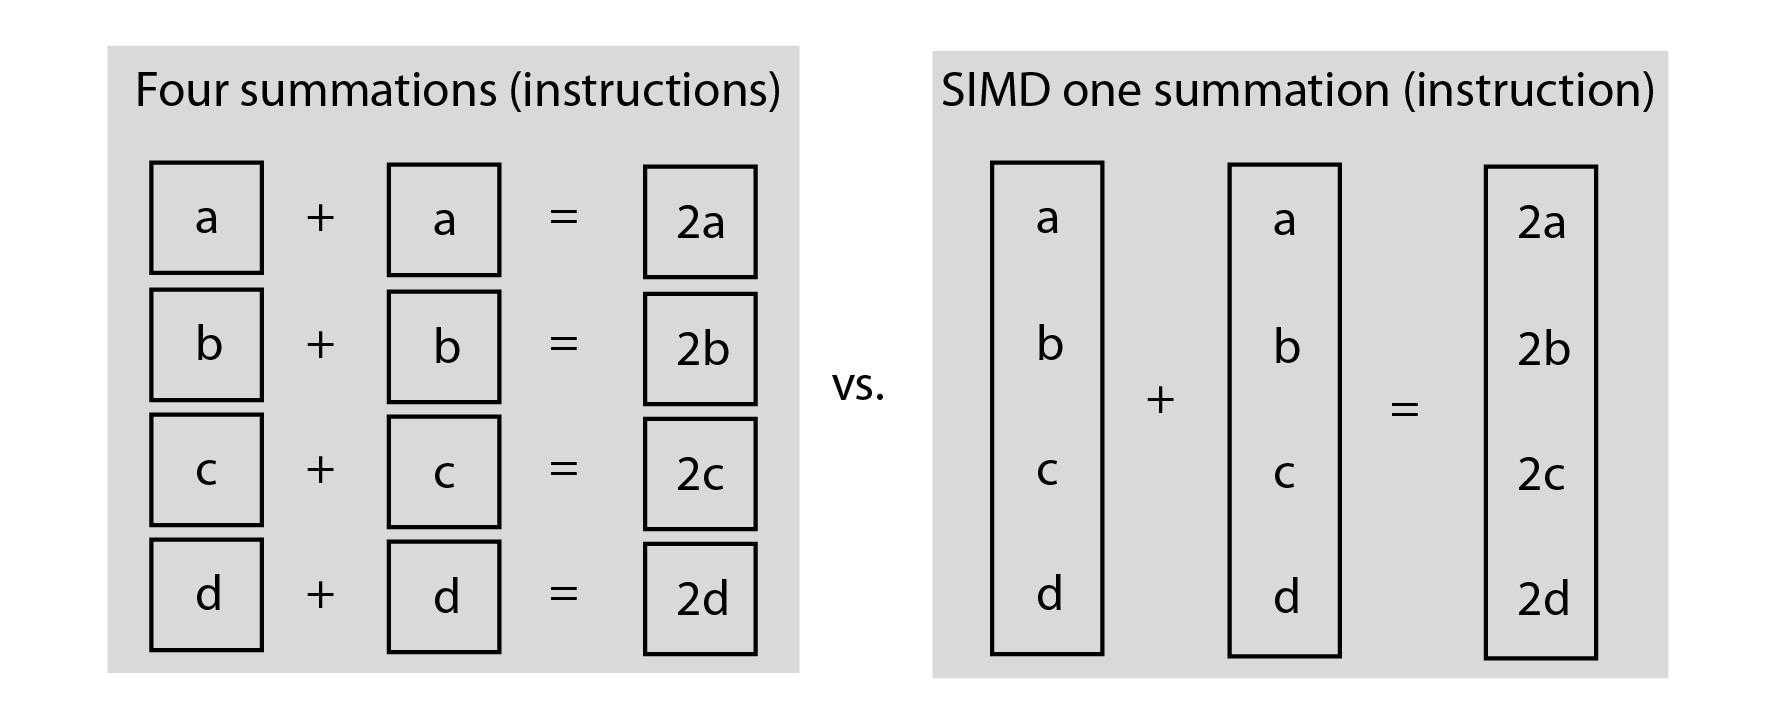
\includegraphics[width=\textwidth]{scalar_vs_simd}
\centering
\captionsetup{justification=centering, singlelinecheck=false}
	\caption{ Πρόσθεση διανυσμάτων βαθμωτά και με \en{SIMD}}
\label{fig:scalar_vs_simd}
\end{figure}
\clearpage
\subsubsection{Η οδηγία \emph{\en{simd}}}
\subparagraph{}
Η οδηγία \emph{\en{simd}} ισχύει για έναν ή περισσότερους βρόγχους. Η δομή του βρόγχου στον οποίο εφαρμόζεται η οδηγία είναι ίδια με την δομή του βρόγχου της \emph{\en{C++}}. Οι φράσεις που υποστηρίζονται είναι οι παρακάτω:
\selectlanguage{english}
\begin{lstlisting}[language=C++, caption={\el{Φράσεις που υποστηρίζονται από} simd} , frame=tlrb]{Name}
private (list)
lastprivate (list)
reduction (reduction-identifier : list)
collapse (n)
simdlen (length)
safelen (length)
linear (list[: linear-step J)
aligned (list{:alignment])
\end{lstlisting}
\selectlanguage{greek}
\ \\
Η προσθήκη της οδηγίας \emph{\en{simd}} δίνει εντολή στο μεταγλωττιστή να δημιουργήσει έναν \emph{\en{simd}} βρόγχο.
Η χρήση δεικτών μέσα στο βρόγχο μπορεί να προκαλέσει απροσδιοριστη συμπεριφορα υπο συνθήκες. Για παράδειγμα, αν ο δείκτης \emph{\en{k}} ή \emph{\en{m}} είναι ταυτόσημος με τον δείκτη t, τότε αναμένεται τα αποτελέσματα να είναι λάθος.
\ \\
\selectlanguage{english}

\begin{lstlisting}[language=C++, caption={\el{Παράδειγμα κώδικα με} simd} , frame=tlrb]{Name}
void accumulate(int *t, int *k, int *m, int n) {
	#pragma omp simd
	for (int i = 0; i < n; ++i) {
		t[i] = k[i] + m[i];
	}
}
\end{lstlisting}
\selectlanguage{greek}

\clearpage
Στο παραπάνω παράδειγμα, η μεταβλητή \emph{\en{i}} είναι ιδιωτική. Η διαφορά με την ιδιωτική μεταβλητή ενός παράλληλου βρόγχου είναι οτι η ιδιωτικότητα αναφέρεται σε ένα \emph{\en{SIMD lane}}. Oι τιμές των διανυσμάτων \emph{\en{t, k, m}} είναι κοινόχρηστες. Ο μεταγλωττιστής επιλέγει το κατάλληλο μήκος του διανύσματος για τη συγκεκριμένη αρχιτεκτονική. 
Οι φράσεις \emph{\en{private, lastprivate, reduction, collapse, ordered}}, έχουν την ίδια χρησιμότητα που προαναφέρθηκε στις παραπάνω οδηγίες (πχ οδηγία διαμοιρασμού βρόγχου).


\paragraph{H φράση \emph{\en{simdlen}}}
\subparagraph{}
Η φράση \emph{\en{simdlen}} δέχεται ως όρισμα ένα θετικό ακέραιο αριθμό που καθορίζει τον προτιμώμενο αριθμό επαναλήψεων ενός βρόγχου που θα εκτελούνται ταυτόχρονα. Επηρεάζει το μήκος του διανύσματος που χρησιμοποιείται από τις παραγόμενες \emph{\en{simd}} οδηγίες.

Η τιμή του ορίσματος είναι προτιμητέα αλλα όχι υποχρεωτική. Ο μεταγλωττιστής έχει την ελευθερία να αποκλίνει από αυτή την επιλογή και να επιλέξει διαφορετικό μήκος. Ελλείψη αυτής της φράσης ορίζεται μια προεπιλεγμένη τιμή που καθορίζεται από την υλοποίηση. Σκοπός της φράσης \emph{\en{simdlen}} είναι να καθοδηγήσει τον μεταγλωττιστή. Χρησιμοποιείται από τον χρήστη όταν έχει καλή εικόνα των χαρακτηριστικών του βρόγχου και γνωρίζει ότι κάποιο συγκεκριμένο μήκος μπορεί να ωφελήσει στην απόδοση.
\ \\

\paragraph{H φράση \emph{\en{safelen}}}
\subparagraph{}
Η φράση \emph{\en{safelen}} δέχεται ως όρισμα ένα θετικό ακέραιο αριθμό. Η τιμή αυτή καθορίζει το ανώτερο όριο του μήκους διανύσματος. Είναι ο αριθμός που στο οποίο είναι ασφαλές για τον βρόγχο. Το τελικό μήκος διανύσματος επιλέγεται από τον μεταγλωττιστή, αλλά δεν υπερβαίνει την τιμή της φράσης 
\emph{\en{safelen}}.

Στο παρακάτω παράδειγμα απαιτείται η φράση \emph{\en{safelen}}. Πρόκειται για έναν βρόγχο που περιέχει
 δέσμευση στην προσπέλαση των στοιχείων του διανύσματος.
 Για παράδειγμα, το διάβασμα του \emph{\en{[i-10]}} στην επανάληψη \emph{\en{i}} δεν μπορεί να γίνει, μέχρι να ολοκληρωθεί ή εγγραφή στο \emph{\en{k[i]}} της προηγούμενης επανάληψης.
 
 \clearpage
 \selectlanguage{english}

\begin{lstlisting}[language=C++, caption={\el{Παράδειγμα κώδικα με} simd} , frame=tlrb]{Name}
void dep_loop(float *k, float c, int n) {
	for (int i=10; i<n; i++) {
		k[i] = k[i-10] * c;
	}
}
\end{lstlisting}
\selectlanguage{greek}

\paragraph{H φράση \emph{\en{linear}}}
\subparagraph{}
Τα βαθμωτά στοιχεία εισέρχονται σε διανύσματα, στα οποία εκτελούνται οδηγίες \emph{\en{simd}} και εξέρχονται. Οταν τα στοιχεία είναι προσβάσιμα με γραμμικό τρόπο, το διάνυσμα κατασκευάζεται εύκολα. Για παράδειγμα, δεδομένου ότι διατηρείται η ευθυγράμμιση των δεδομένων, μια απλή \emph{\en{simd}} οδηγία φόρτωσης και αποθήκευσης, χρησιμοποιείται για να γράψει και να διαβάσει διαδοχικά δεδομένα στο διάνυσμα.

Σε περιπτώσεις που τα βαθμωτά παρατίθενται διαδοχικά στη μνήμη, η πρόσβαση στα στοιχεία γίνεται με \emph{μοναδιαίο βήμα}. Αν τα δεδομένα δεν είναι διατεταγμένα σε διαδοχικές θέσεις μνήμης, αλλά με  κάποια μετατόπιση μεταξύ τους, τότε η προσέγγιση του μπορεί να γίνει με μεγαλύτερο βήμα. Στην περίπτωση αυτή το βήμα είναι ίσο με τη μετατόπιση μεταξύ των στοιχείων.

\begin{figure}[h]
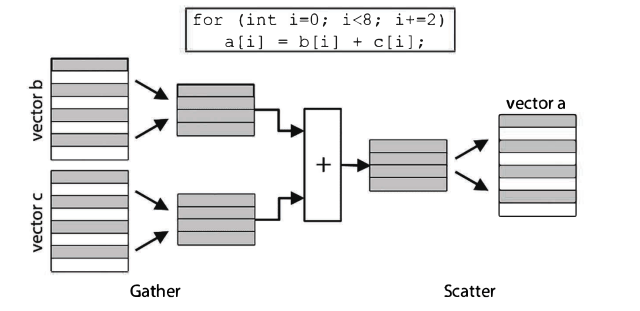
\includegraphics[width=0.9\textwidth]{linear_clause_simd}
\centering
\captionsetup{justification=centering, singlelinecheck=false}
	\caption{Σχηματική απεικόνιση φράσης \emph{\en{linear}}}
\label{fig:linear_clause_simd}
\end{figure}

Για την κατασκευή του διανύσματος, μια λειτουργία συγκέντρωσης διαβάζει γραμμικά αλλά με βήμα μεγαλύτερο του ενός. Ομοίως, μια λειτουργία γράφει τα δεδομένα του διανύσματος πίσω στη μνήμη γραμμικά, αλλα με βήμα μεγαλύτερο του ενος.


\paragraph{H φράση \emph{\en{aligned}}}
\subparagraph{}
Η ευθυγράμμιση των δεδομένων είναι σημαντική για την καλή απόδοση του προγράμματος. Εαν ένα στοιχεία δεν είναι ευθυγραμμισμένο σε διευθυνση μνήμης που είναι πολλαπλάσιο του μεγέθους του στοιχείου σε byte, προκύπτει ένα επιπλέον κόστος  κατά την πρόσβαση στο στοιχείο αυτό.

Για παράδειγμα, σε ορισμένες αρχιτεκτονικές ενδέχεται να μην είναι δυνατή η φόρτωση και εγγραφή απο μια διεύθυνση μνήμης που δεν ειναι ευθυγραμμισμένη με το μέγεθος του δεδομένου που χρησιμοποιείται. Αν ισχύει κάτι τέτοιο, οι λειτουργίες γίνονται κανονικά, με μεγαλύτερο κόστος. Σε περίπτωση διανυσματοκοποίησης μέσω της χρήσης οδηγίας \emph{\en{simd}}, αλλά η προκύπτουσα απόδοση είναι κακή, η προσαρμογή ευθυγράμμισης δεδομένων μπορεί να βελτιώσει την εκτέλεση.

Η φράση ευθυγράμμισης υποστηρίζεται τόσο από την οδηγία \emph{\en{simd}} όσο και από την οδηγία \emph{\en{declare simd}}. Η φράση δέχεται ως όρισμα μια λίστα μεταβλητών. Η ευθυγράμμιση πρέπει να είναι ενας σταθερός ακεραιος αριθμός. Σε περίπτωση έλλειψης της φράσης, μια προεπιλεγμένη τιμή καθορίζεται από την υλοποίηση.

\paragraph{Η σύνθετη οδηγία βρόγχου \emph{\en{SIMD}}}
\subparagraph{}

\selectlanguage{english}
\begin{lstlisting}[language=C++, caption={\el{Παράδειγμα κώδικα με} simd} , frame=tlrb]{Name}
#pragma omp for simd [clause[[,] clause] ...] new-line
	for-loops
\end{lstlisting}
\selectlanguage{greek}

\ \\
Η σύνθετη οδηγία βρόγχου \emph{\en{SIMD}}, συνδυάζει παραλληλισμό νημάτων και \emph{\en{SIMD}}. Κομμάτια επαναλήψεων βρόγχου διανέμονται στα νήματα σε μια ομάδα. Στη συνέχεια εκτελούνται τα κομμάτια των επαναλήψεων με βρόγχο \emph{\en{simd}}. Μια φράση που μπορεί να εμφανιστεί στην οδηγία διαμοιρασμού βρόγχου είτε στην οδηγία \emph{\en{simd}} μπορεί να εμφανιστεί και στο σύνθετο όρο.

Στη σύνθετη οδηγία, τμήματα επαναλήψεων του βρόγχου κατανέμονται σε μια ομάδα νημάτων με τη μέθοδο που ορίζεται από τις φράσεις που ορίζονται και για την οδηγία διαμοιρασμού βρόγχου. Στη συνέχεια, τα κομμάτια επαναλήψεων βρόγχου μπορούν να μετατραπούν σε οδηγίες \emph{\en{simd}} με μέθοδο που καθορίζεται από της φράσης που ορίζεται και για την οδηγία \emph{\en{simd}}. Τα παραπάνω φαίνονται σχηματικά στην επόμενη εικόνα:
\ \\
\begin{figure}[h]
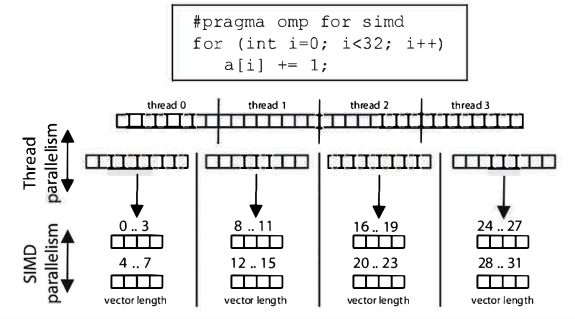
\includegraphics[width=0.9\textwidth]{for_simd}
\centering
\captionsetup{justification=centering, singlelinecheck=false}
	\caption{ Βήματα διεργασιών οδηγίας \emph{\en{for simd}}}
\label{fig:for_simd}
\end{figure}

Κάθε βρόγχος έχει ένα συγκεκριμένο ποσοστό εργασίας που πρέπει να εκτελέσει. Αν ο αριθμός των νημάτων αυξηθεί, το ποσοστό της εργασίας ανα νήμα θα μειωθεί. Προσθέτοντας παραλληλισμό \emph{\en{simd}}, δεν ειναι απραίτητη η βελτίωση της απόδοσης, ειδικά αν ο simd βρόγχος που ανήκει σε ένα νήμα, μειώσει το μήκος του.
\clearpage{}
\subsubsection{Συναρτήσεις \emph{\en{SIMD}}}
\subparagraph{}
Οι κλίσεις συναρτήσεων εντός βρόγχου \emph{\en{simd}} εμποδίζουν τη δημιουργία αποτελεσματικών \emph{\en{simd}} δομών. Στη χειρότερη περίπτωση η κλήση της συνάρτησης θα γίνει χρησιμοποιώντας βαθμωτά δεδομένα, και πιθανότατα θα επηρεάσει αρνητικά την αποτελεσματικότητα.

Για την πλήρη εκμετάλλευση του παραλληλισμού SIMD, μια συνάρτηση που καλείται μέσα από ένα βρόγχο \emph{\en{simd}}, πρέπει να έιναι σε μια ισοδύναμη έκδοση  της συνάρτησης \emph{\en{simd}}. Ετσι, ο μεταγλωτιστής πρέπει να δημιουργήσει αυτή την ειδική έκδοση της συνάρτησης αυτής με \emph{\en{simd}} παραμέτρους και οδηγίες.

Η οδηγία \emph{\en{simd directive}} χρησιμοποιείται για να δημιουργήσει ο μεταγλωττιστής μια ή περισσότερες \emph{\en{simd}} εκδόσεις μιας συνάρτησης. Αυτές οι εκδόσεις χρησιμοποιούνται απο βρόγχους \emph{\en{simd}}.



\paragraph{H οδηγία \emph{\en{declare simd}}}
\subparagraph{}
Η οδηγία \emph{\en{declare simd}} χρησιμοποιείται για να δηλώσει οτι μια \emph{\en{simd}} παραλλαγή μιας συνάρτησης μπορεί να χρησιμοποιηθεί από μια περιοχή παραλληλισμού \emph{\en{simd}}.

\selectlanguage{english}
\begin{lstlisting}[language=C++, caption={\el{Χρήση οδηγίας} declare simd} , frame=tlrb]{Name}
#pragma omp declare simd [clause [[,] clause] ...] new-line
 function declaration definitions
\end{lstlisting}
\selectlanguage{greek}

\selectlanguage{english}
\begin{lstlisting}[language=C++, caption={\el{Φράσεις που υποστηρίζονται από} simd} , frame=tlrb]{Name}
simdlen (length)
linear (list[: linear-step J)
aligned (list[:alignmentj)
uniform ( argument-list)
inbranch
notinbranch
\end{lstlisting}
\selectlanguage{greek}

Ο μεταγλωττιστής μπορεί να δημιουργήσει πολλές εκδόσεις μιας συνάρτησης \emph{\en{simd}} και να επιλέξει την κατάλληλη για να κληθεί σε μια συγκεκριμένη τοποθεσία μιας κατασκευής \emph{\en{simd}}. Ο χρήσης μπορεί να προσαρμόσει την λειτουργία μιας συνάρτησης με εξειδικευμένες φράσεις.

Υπάρχουν δύο περιορισμοί. Αν μια μεταβλητή αλλάζει ως αποτέλεσμα μιας τροποποίησης μιας φαινομενικά άσχετης μεταβλητής η συμπεριφορά είναι απροσδιόριστη. Επιπλέον, μια συνάρτηση που εμφανίζεται κάτω απο οδηγία \emph{\en{declare simd}}, δεν επιτρέπονται τα \emph{\en{exceptions}}.



Μια παρενέργεια στο πλαίσιο του προγραμματισμού λέγεται ότι συμβαίνει εάν μια μεταβλητή
αλλάζει ως αποτέλεσμα μιας τροποποίησης σε μια φαινομενικά άσχετη μεταβλητή. Αυτό
μπορεί να συμβεί λόγω του ψευδώνυμου του δείκτη για παράδειγμα. Σε μια τέτοια κατάσταση, δύο
διαφορετικοί δείκτες δείχνουν στην ίδια θέση μνήμης. Αλλαγή ενός δείκτη
επηρεάζει τους άλλους. Ένα άλλο παράδειγμα είναι μια συνάρτηση που τροποποιεί τα παγκόσμια δεδομένα.
Δεδομένου ότι τα παγκόσμια δεδομένα χρησιμοποιούνται (δυνητικά) από άλλες λειτουργίες, αυτό μπορεί να προκαλέσει καταστροφή
σε ένα παράλληλο πρόγραμμα και πρέπει να ληφθεί μέριμνα για την αντιμετώπιση αυτής της κατάστασης.


\paragraph{Χαρακτηριστικά παραμέτρων συνάρτησης \emph{\en{simd}}}
\subparagraph{}
Οι φράσεις \emph{\en{uniform, linear, simdlen, aligned}} χρησιμοποιούνται για τον καθορισμό χαρακτηριστικών για τις παραμέτρους της συνάρτησης \emph{\en{simd}}. Εκτός από τη ρήτρα \emph{\en{simdlen}}, οι μεταβλητές που εμφανίζονται στις υπόλοιπες φράσεις πρέπει να είναι παράμετροι της συνάρτησης για την οποία ισχύει η οδηγία.

Οταν μια παράμετρος βρίσκεται στη φράση \emph{\en{uniform}}, υποδεικνύει οτι η τιμή της παραμέτρου έχει την ίδια τιμή για όλες τις ταυτόχρονες κλήσεις κατά την εκτέλεση μιας οδηγίας \emph{\en{simd}} βρόχου.
Η φράση \emph{\en{linear}} έχει διαφορετική σημασία όταν εμφανίζεται σε οδηγία \emph{\en{simd}}. Δείχνει οτι ένα όρισμα που μεταβιβάζεται σε μια συνάρτηση έχει γραμμική σχέση μεταξύ των παράλληλων επικλήσεων μιας συνάρτησης.

Κάθε \emph{\en{simd}} λωρίδα παρατηρεί την τιμή του ορίσματος στην πρώτη λωρίδα και προσθέτει την μετατόπιση της \emph{\en{simd}} λωρίδας από την πρώτη, επί το γραμμική βήμα.
$$val_{curr} = val_1 + offset * step $$

Η φράση \emph{\en{uniform(arg1, arg2)}} ενημερώνει τον \emph{\en{compiler}} να δημιουργήσει μια \emph{\en{simd}} συνάρτηση που προυποθέτει οτι αυτές οι δύο μεταβλητές είναι ανεξάρτητες από τον βρόγχο.

Η φράση \emph{\en{inbranch}} υποστηρίζει οτι μια συνάρτηση καλείται πάντα μέσα σε ένα βρόγχο \emph{\en{simd}} που περιέχει \emph{\en{if condition}}. Ο μεταγλωττιστής πρέπει να αναδιαρθρώσει τον κώδικα για να χειριστεί την πιθανότητα ότι μια λωρίδα \emph{\en{simd}} μπορεί να μην εκτελέσει τον κώδικα μιας συνάρτησης.

Η φράση \emph{\en{notinbranch}} χρησιμοποιείται όταν η συνάρτηση δεν εκτελείται ποτέ μέσα από ένα \emph{\en{if condition}} σε ένα \emph{\en{simd}} βρόγχο. Επιτρέπει τον μεταγλωττιστή κάνει μεγαλύτερες βελτιστοποιήσεις στην απόδοση του κώδικα μιας συνάρτησης που χρησιμοποιεί \emph{\en{simd}} οδηγίες.

\selectlanguage{english}
\begin{lstlisting}[language=C++, caption={\el{ Παράδειγμα χρήσης φράσεων} inbranch - notinbranch} , frame=tlrb]{Name}
#pragma omp declare simd inbranch
float pow(float x) {
	return (x * x);
}

#pragma omp declare simd notinbranch
extern float div(float);

void simd_loop(float *a, float *b, int n)
{
	#pragma omp simd
	for (int i=0; i<n; i++) {
		if (a[i] < 0.0 )
			b[i] = pow(a[i]);
		b[i] = div(b[i]);
	}
}
\end{lstlisting}
\selectlanguage{greek}

\clearpage
\subsection{\en{Thread Affinity}}
\subparagraph{}
\emph{\en{Thread Affinity}} είναι μια ευρύτερη έννοια που περιλαμβάνει την βελτιστοποίηση του χρόνου εκτέλεσης ενός προγράμματος, μέσω βελτιστοποιήσεων στο εύρος ζώνης μνήμης, τη ν αποφυγή καθυστέρησης μνήμης ή της  καθυστέρησης χρήσης προσωρινής μνήμης.

To \emph{\en{OpenMP 4.0}} εισάγει ένα σύνολο οδηγιών για την υποστήριξη του \emph{\en{thread affinity}}\cite{thread_affinity}. Η πλειοψηφία πλέον των μηχανημάτων βασίζονται στην \emph{\en{cc-NUMA}} αρχιτεκτονική. Ο λόγος που αυτό το σύστημα μνήμης έγινε κυρίαρχο, είναι η συνεχής αύξηση του αριθμού των επεξεργαστών. Η μονολιθική διασύνδεση μνήμης με σταθερό εύρος ζώνης μνήμης θα αποτελούσε πρόβλημα στην ραγδαία αύξηση των επεξεργαστών.

Στη \emph{\en{cc-NUMA}} αρχιτεκτονική κάθε υποδοχή συνδέεται με ένα υποσύνολο της συνολικής μνήμης του συστήματος. Μία διασύνδεση ενώνει τα υποσύνολα μεταξύ τους και δημιουργεί την εικόνα ενιαιας μνήμης στον χρήστη. Ενα τέτοιο σύστημα είναι ευκολότερο να επεκταθεί.

Το πλεονέκτημα της διασύνδεσης είναι ότι η εφαρμογή έχει πρόσβαση σε όλη την μνήμη του συστήματος, ανεξάρτητα από το που βρίσκονται τα δεδομένα. Ωστόσο, πλεον ο χρόνος πρόσβασης σε αυτά δεν ειναι ο σταθερός καθώς εξαρτάται από τη θέση τους στη μνήμη.


\begin{figure}[h]
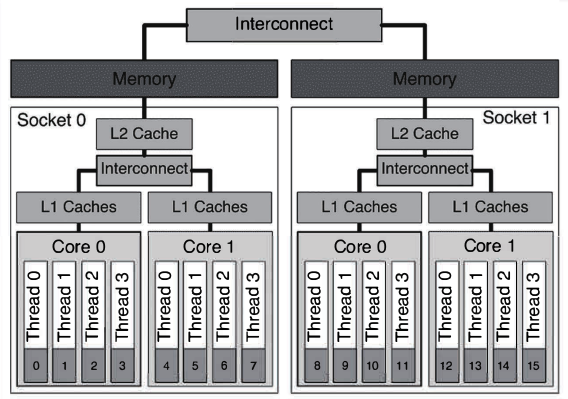
\includegraphics[width=0.75\textwidth]{numa}
\centering
\captionsetup{justification=centering, singlelinecheck=false}
	\caption{Αρχιτεκτονική \en{cc-NUMA}\cite{thenextstep152}}
\label{fig:numa}
\end{figure}



\subsection{\en{Tasking}}
\subparagraph{}
Η έννοια των διεργασιών (\emph{\en{Tasking}}) εισήχθει στο \en{OpenMP} το 2008 με την έκδοση 3.0\cite{parallel_dist}.
Οι διεργασίες παρέχουν τη δυνατότητα, οι αλγόριθμοι με ακανόνιστη και εξαρτώμενη από το χρόνο ροή εκτέλεσης να μπορούν να παραλληλιστούν. Ένας μηχανισμός ουράς διαχειρίζεται δυναμικά την εκχώρηση νημάτων στη διεργασία που πρέπει να εκτελεστεί. Τα νήματα παραλαμβάνουν εργασίες από την ουρά εως ότου αυτή αδειάσει.
Διεργασία (\emph{\en{task}}) είναι ενα μπλοκ κώδικα σε μια παράλληλη περιοχή που εκτελειται ταυτόχρονα με μια αλλη διεργασία στην ίδια περιοχή. 

Οι διεργασίες είναι τμήμα της παράλληλης περιοχής.
Χωρίς ειδική μέριμνα, η ίδια διεργασία μπορεί να εκτελεστεί από διαφορετικά νήματα. Αυτό αποτελεί ασάφεια, καθώς οι οδηγίες διαμοιρασμού μνήμης, καθορίζουν με σαφήνεια τον τρόπο που οι εργασίες διανέμονται στα νήματα. Για να εγγυηθεί το \en{OpenMP} ότι κάθε διεργασία εκτελείται μόνο μια φορά, η κατασκευή τους θα πρέπει να ενσωματωθούν σε μια οδηγία \emph{\en{single}} ή \emph{\en{master}}.

		\selectlanguage{english}
		\begin{lstlisting}[tabsize=4, basicstyle=\small, language=C++, caption={\el{Παράδειγμα κώδικα με διεργασίες}}, frame=tb]
#include <omp.h>

int main(void) {	
	#pragma omp parallel          // Begin of parallel region
	{
		#pragma omp single
		{
			#pragma omp task
				func_task_1();    // First task creation
			#pragma omp task
				func_task_2();    // Second task creation
		}// end of single region  // Implicit barrier
	} //end of parallel region    // Implicit barrier
}
\end{lstlisting}
\selectlanguage{greek}
\clearpage
Το παραπάνω παράδειγμα αποτελεί επεξήγηση της λειτουργίας των διεργασιών. Υπάρχουν δύο νήματα, ένα νήμα συναντά την οδηγία \emph{\en{single}} και αρχίζει να εκτελεί το μπλοκ κώδικα. Δύο διεργασίες δημιουργούνται, αλλά δεν έχουν ακόμη εκτελεστεί. Tο άλλο νήμα συναντά και περιμένει στο  \emph{\en{barrier}} στο τέλος της οδηγίας \emph{\en{single}}. Στην περίπτωση την διεργασιών, τα αδρανή νήματα δεν περιμένουν στο \emph{\en{barrier}}. Αντι αυτου, αυτά τα νήματα είναι διαθέσιμα για την εκτέλεση των διεργασιών. Το νήμα που δημιουργεί τις διεργασίες καταλήγει επίσης στο φράγμα, μόλις ολοκληρωθεί η φάση παραγωγής και μπορεί να εκτελεί και αυτό διεργασίες. Η σειρά με την οποία θα εκτελεστούν οι διεργασίες δεν καθορίζεται.

\subsubsection{Η οδηγία διεργασιών}
\subparagraph{}
	Ορίζει μια ρητή διεργασία. Το περιβάλλον δεδομένων της διεργασίας δημιουργείται σύμφωνα με τις φράσεις χαρακτηριστικών κοινής χρήσης δεδομένων κατασκευή διεργασίων και τυχόν προεπιλογές που ισχύουν\cite{thenextstep20}.
	
\selectlanguage{english}
\begin{lstlisting}[language=C++, caption={\el{Σύνταξη διεργασίας}} , frame=tlrb]{Name}
		#pragma omp task [clause[ [, ]clause] ...] 
			structured-block 
\end{lstlisting}

\begin{lstlisting}[language=C++, caption={\el{Αποδεκτές φράσεις οδηγίας} sections} , frame=tlrb]{Name}
if([ task :] scalar-expression) 
final(scalar-expression) 
untied 
default(shared | none) 
mergeable 
private(list) 
firstprivate(list) 
shared(list) 
in_reduction(reduction-identifier : list) 
depend([depend-modifier,] dependence-type : locator-list) 
priority(priority-value) 
allocate([allocator :] list) 
affinity([aff-modifier :] locator-list) 
detach(event-handle)
\end{lstlisting}
\selectlanguage{greek}

\paragraph{Φράση \en{if}}
\subparagraph{}
Η έκφραση της συνθήκης \emph{\en{if}} μιας διεργασίας, θα πρέπει να αξιολογείται ώς ψευδής ή αληθής. 
Η οδηγία των διεργασιών παρέχει μια φράση \emph{\en{if}}, που δέχεται μια έκραση ως όρισμα. Αν η έκφραση αξιολογείται ώς ψευδής, απαγορεύει η αναβολή της διεργασίας.
Ανεξαρήτου αποτελέσματος της έκφρασης, δημιουργείται πάντα ένα νέο περιβάλλον δεδομένων εργίας. Αν η έκφραση αξιολογείται ως ψευδής, δεν γίνονται όλοι οι υπολογισμοί που απετούνται για μια διεργασία αν δεν υπήρχε η φράση if, επομένως θα μπορούσαν να αποφευχθούν ορισμένα κόστη επιδόσεων.

Ως εκ τούτου η φράση \emph{\en{if}} αποτελεί λύση σε καταστάσεις, όπως οι αναδρομικοί αλγόριθμοι, όπου
το υπολογιστικό κόστος μειώνεται καθώς αυξάνεται το βάθος και το όφελος από τη δημιουργία μιας νέας διεργασίας
μειώνεται λόγω του γενικού κόστους.
Ωστόσο, για λόγους ασφαλείας \cite{parallel_dist}, οι μεταβλητές που αναφέρονται σε μια οδηγία κατασκευής διεργασιών είναι, στις περισσότερες περιπτώσεις, από προεπιλογή \emph{\en{firstprivate}}, επομένως το κόστος
της ρύθμισης περιβάλλοντος δεδομένων μπορεί να είναι το κυρίαρχο συστατικό της δημιουργίας διεργασιών.

\paragraph{Φράση \en{final}}
\subparagraph{}
Η φράση χρησιμοποιείται για να ελέγχεται με ευκρίνεια η ευαισθησία των διεργασιών. Οταν χρησιμοποιείται μέσα στην οδηγεία \emph{\en{task}}, η έκφραση αξιολογείται κατά τη διάρκεια δημιουργίας αυτού.  Αν είναι αληθής, η διεργασία θεωρείται τελική. Όλες οι διεργασίες που δημιουργούνται μέσα σε αυτή τη διεργασία, αγνοούνται και εκτελούνται στο πλαίσιο της.
\clearpage
Υπάρχουν δυο διαφορές ανάμεσα στη φράση \emph{\en{if}} και στη \emph{\en{final}}: την κατασκευή διεργασιών που επηρεάζει και τον τρόπο με τον οποίο οι κατασκευές αγνοούνται\cite{tasking1}.

\begin{table}[htbp]
\captionsetup{justification=raggedright,
singlelinecheck=false
}
\caption{Διαφορές ανάμεσα στις φράσεις \emph{\en{if}} και \emph{\en{final}} οταν εισάγονται σε κατασκευή διεργασίας.}
\def\arraystretch{1.5}
\begin{tabular}{| p{0.5\textwidth} | p{0.5\textwidth}|}
\textbf{\en{\emph{if} clause}} \cellcolor[HTML]{D0D0D0} & \textbf{\en{\emph{final} clause}} \cellcolor[HTML]{D0D0D0} \\
\hline
Επηρεάζει την διεργασία που κατασκευάζεται από τη συγκεκριμένη οδηγιά κατασκευής διεργασιών & Επηρεάζει όλες τις διεργασίες "απογόνους" δηλαδή όλες τις διεργασίες που πρόκειται να δημιουργηθούν μέσα από αυτή που περιείχε τη φράση \emph{\en{final}}\\
\hline
Η οδηγία κατασκευής διεργασίας αγνοείται εν μέρει. Η διεργασία και το περιβάλλον μεταβλητών δημιουργείται ακόμα και αν η έκφραση αξιολογηθεί ως \emph{\en{false}} & Αγνοείται εντελώς η κατασκευή διεργασιών δηλαδή δε θα δημιουργηθεί νέα εργασία ούτε νέο περιβάλλον δεδομένων.	\\
\hline
\end{tabular}
\end{table}

\paragraph{Φράση \en{mergeable}}
\subparagraph{}

Μια συγχωνευμένη διεργασία είναι η διεργασία της οποίας το περιβάλλον δεδομένων είναι ίδιο με το περιβάλλον που δημιούργησε την διεργασία. Οταν εισάγεται η φράση \emph{\en{mergeable}} σε μια οδηγία δημιουργίας διεργασίας τότε η υλοποίηση μπορεί να δημιουργήσει μια συγχωνευμένη διεργασία.

\paragraph{Φράση \en{depend}}
\subparagraph{}

Η φράση \emph{\en{depend}} επιβάλλει πρόσθετους περιορισμούς στη δημιουργία διεργασιών. Αυτοί οι περιορισμοί δημιουργούν εξαρτήσεις μόνο μεταξύ συγκενικών διεργασιών.
\clearpage

\paragraph{Φράση \en{untied}}
\subparagraph{}
Κατά την επανάληψη μιας περιοχής διεργασίας που έχει τεθεί σε αναστολή, μια δεσμευμένη διεργασία θα πρέπει να εκτελεστεί ξανά από το ίδιο νήμα. Με τη φράση \emph{\en{untied}}, δεν υπάρχει τέτοιος περιορισμός και η διεργασία συνεχίζεται από οποιοδήποτε νήμα.


\ \\
\subsubsection{Συγχρονισμός διεργασιών}
\subparagraph{}
Οι διεργασίες δημιουργούνται όταν υπάρχει μια οδηγία δημιουργίας διεργασιών. Η στιγμή εκτέλεσης τους δεν είναι καθορισμένη. Το \emph{\en{OpenMP}} εγγυάται οτι θα έχουν ολοκληρωθεί όταν ολοκληρωθεί η εκτέλεση του προγράμματος, ή όταν προκύψει κάποια οδηγία συγχρονισμού διεργασίας.
\ \\
\ \\

\begin{table}[htbp]
\captionsetup{justification=raggedright,
singlelinecheck=false
}
\caption{Οδηγιες συγχρονισμού διεργασιών.}
\def\arraystretch{1.5}
\begin{tabular}{| p{0.5\textwidth} | p{0.5\textwidth}|}
\textbf{Οδηγία} \cellcolor[HTML]{D0D0D0} & \textbf{Περιγραφή} \cellcolor[HTML]{D0D0D0} \\
\hline
\textbf{\en{{\#}pragma omp barrier}} & Μπορεί είτε να υπάρχει υπονοούμενη είτε να δηλωθεί ρητά. \\
\hline
\textbf{\en{{\#}pragma omp taskwait}} & Περιμένει μέχρι να ολοκληρωθούν όλες οι διεργασίες παιδιά της συγκεκριμένης διεργασίας.\\
\hline
\textbf{\en{{\#}pragma omp taskgroup}} & Περιμένει μέχρι να ολοκληρωθούν όλες οι διεργασίες παιδιά της συγκεκριμένης διεργασίας αλλά και οι απόγονοι τους.\\
\hline
\end{tabular}
\end{table}

Στην περίπτωση της δημιουργίας διεργασιών μέσω οδηγίας single, υπάρχει υπονοούμενο φράγμα εκτέλεσης, σε αντίθεση με την οδηγία master που δεν υπονοείται.
\clearpage
\selectlanguage{english}
\begin{lstlisting}[language=C++, caption={\el{Παράδειγμα} taskwait} , frame=tlrb]{Name}
#pragma omp parallel {
	#pragma omp single
	{
		#pragma omp task
		{
			function1();
		}//Task #1
		#pragma omp task
		{
			function2();
		} // Task #2

		#pragma omp taskwait
			last_to_be_executed();
	} // End of single region
} // End of parallel region
\end{lstlisting}
\selectlanguage{greek}
\clearpage
\subsection{Ετερογενής Αρχιτεκτονική}
\subparagraph{}
Η ετερογενής αρχιτεκτονική είναι ένα σύνολο προδιαγραφών που επιτρέπουν την ενσωμάτωση κεντρικών μονάδων επεξεργασίας και επεξεργαστών γραφικών στον ίδιο δίαυλο, με κοινόχρηστη μνήμη και διεργασίες\cite{toms_hardware}.

Εξειδικευμένη επεξεργαστές επιταχυντών που βελτιώνουν δραματικά την απόδοση υπολογισμών, πολλαπλασιάζονται και οι επεξεργαστές γενικής χρήσης συνδέονται σε κάποιον επιταχυντή. Η αύξηση της δημοτικότητας αυτών των ετερογενών αρχιτεκτονικών σε όλους τους τύπους υπολογιστών είχε αξιοσημείωτο αντίκτυπο στην ανάπτυξη λογισμικού.

Για την εκμετάλλευση αυτών των συστημάτων, οι χρήστες πρέπει να κατασκευάζουν λογισμικό που εκτελεί διάφορες περιοχές κώδικα σε διαφορετικούς τύπους συσκευών. Το μεγαλύτερο κίνητρο αποτελεί η επιτάχυνση των υπολογισμών στους βρόγχους επανάληψης.

Ωστόσο, τα μοντέλα προγραμματισμού για αυτά τα συστήματα είναι δύσκολο να χρησιμοποιηθούν. Συχνά, οι ενότητες κώδικα γράφονται δύο φορές, μία φορά για τον επεξεργαστή γενικού σκοπού και μια για τον επιταχυντή. Η έκδοση του επιταχυντή γράφεται γλώσσα χαμηλότερου επιπέδου.
Τα παραπάνω προβλήματα οδηγούν σε δυσκολία συντήρησης λογισμικού και ανάγκη διατήρησης δύο εκδόσεων ίδιου κώδικα.

Για τις ανάγκες διευκόλυνσης, το \emph{\en{OpenMP}} επέκτεινε τις λειτουργίες του με σκοπό να υποστηρίξει αυτούς τους τύπους συστημάτων\cite{barbara}. Τα αποτελέσματα της εργασίας αρχικά δημοσιεύτηκαν στην έκδοση 4.0 και στη ανανεώθηκαν στην έκδοση 4.5.

Ο χρήστης μπορεί να χρησιμοποιήσει την διεπαφή \emph{\en{OpenMP}}, για να προγραμματίσει επιταχυντές σε υψηλότερο επίπεδο γλώσσας και για τη διατήρηση μίας μόνο έκδοσης του κώδικα, η οποία μπορεί να τρέξει είτε σε επιταχυντή είτε σε επεξεργαστή γενικής χρήσης.

Κίνητρο για την εκτέλεση κώδικα σε μια ετερογενή αρχιτεκτονική είναι να εκτελεστεί ένα κομμάτι κώδικα σε έναν επιταχυντή. Ο ρόλος των επιταχυντών είναι η δραματική βελτίωση της απόδοσης ενός προγράμματος αξιοποιώντας τις δυνατότητες υλικού των συσκευών αυτών. Το \emph{\en{OpenMP}} παρέχει τα μέσα για τη διανομή εκτέλεσης ενός προγράμματος σε διαφορετικές συσκευές με ετερογενή αρχιτεκτονική. Συσκευή είναι ένας υπολογιστικός πόρος όπου μια περιοχή κώδικα μπορεί να εκτελεστεί. Παραδείγματα τέτοιων συσκευών είναι GPU, CPU, DSP, FPGA κ.α.

Οι συσκευές έχουν τα δικά τους νήματα, των οποίων η μετεγκατάσταση σε άλλες συσκευές δεν είναι δυνατή. Η εκτέλεση του προγράμματος ξεκινάει από την κεντρική συσκευή (\emph{\en{host device}}. Η κεντρική συσκευή είναι υπέυθυνη για την μεταφορά του κώδικα και των δεδομένων στον επιταχυντή.

\selectlanguage{english}
\begin{lstlisting}[language=C++, caption={\el{Παράδειγμα} taskwait} , frame=tlrb]{Name}
 void add_arrays(double *A, double *B, double *C, size_t size) {
     size_t i = 0;
 #pragma omp target map(A, B, C)
     for (i = 0; i < size; ++i) {
             C[i] = A[i] + B[i];
     }
 }
\end{lstlisting}
\selectlanguage{greek}

Οταν ένα νήμα του εξυπηρετητή συναντάει την οδηγία \emph{\en{target}}, η περιοχή που ακολουθεί εκτελείται σε έναν επιταχυντή. Απο προεπιλογή, το νήμα που συναντά την οδηγία περιμένει την ολοκλήρωση της εκτέλεσης της παράλληλης περιοχής, προτού συνεχίσει.

Πριν το νέο νήμα αρχίσει να εκτελεί την παράλληλη περιοχή, οι μεταβλητές  \emph{\en{A, B, C}} αντιστοιχίζονται στον επιταχυντή. Η φράση \emph{\en{mapped}} είναι η έννοια που χρησιμοποιεί το \emph{\en{OpenMP}} για να περιγράψει τον τρόπο κοινής χρήσης των μεταβλητών σε όλες τις συσκευές.



\subsubsection{Το αρχικό νήμα της συσκευής προορισμού}
\subparagraph{}
Το νήμα που ξεκινάει την εκτέλεση ενός προγράμματος και όλου του σειριακού τμήματος του κώδικα, ονομάζεται κύριο νήμα.
Στην περίπτωση του ετερογενούς προγραμματισμού, το κύριο νήμα ανήκει στην κεντρική συσκευή, δηλαδή το πρόγραμμα ξεκινάει να εκτελείται στην κεντρική συσκευή. 

Με την εισαγωγή της οδηγίας \emph{\en{target}} στο \emph{\en{OpenMP}} 4.0, πολλαπλά αρχικά νήματα μπορούν να δημιουργηθούν κατά τη διάρκεια εκτέλεσης ενός προγράμματος. Την εκτέλεση του τμήματος κώδικα στη συσκευή προορισμού, την αναλαμβάνει ένα νέο αρχικό νήμα και όχι το νήμα που συνάντησε το \emph{\en{target}}. Το νήμα αυτό μπορεί να συναντήσει οδηγίες παραλληλισμού και να δημιουργήσει υποομάδες νημάτων.

\begin{figure}[h]
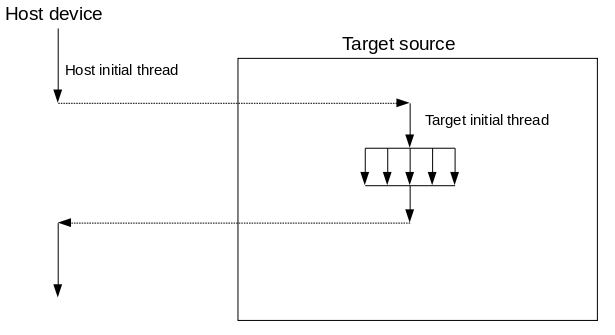
\includegraphics[width=\textwidth]{heter_1}
\centering
\captionsetup{justification=centering, singlelinecheck=false}
	\caption{Διάγραμμα ομάδων νημάτων σε ετερογενή αρχιτεκτονική}
\label{fig:heter_1}
\end{figure}

\subsubsection{H οδηγία \emph{\en{target teams}}}
\subparagraph{}
Η οδηγία \emph{\en{target teams}} κατασκευάζει μια ομάδα (\emph{\en{league}} που λειτουργούν σε έναν επιταχυντή. Κάθε μία από αυτές τις ομάδες είναι ένα αρχικό νήμα που εκτελεί παράλληλα την επόμενη δήλωση κώδικα. Η λειτουργία αυτή είναι παρόμοια με μια οδηγία \emph{\en{parallel}} με τη διαφορά ότι τώρα κάθε νήμα είναι μια ομάδα. Τα νήματα σε διαφορετικές ομάδες δεν μπορούν να συγχρονιστούν μεταξύ τους.

Όταν μια παράλληλη περιοχή συναντάται από μια ομάδα, κάθε αρχικό thread ομάδας γίνεται κύριο σε μια νέα υποομάδα. Το αποτέλεσμα είναι ένα σύνολο υποομάδων, οπου κάθε υποομάδα αποτελείται από ένα ή περισσότερο νήματα.

Αυτή η δομή χρησιμοποιείται για να εκφράζεται ένας τύπος χαλαρού παραλληλισμού, όπου ομάδες νημάτων εκτελούν παράλληλα, αλλά με μικρή αλληλεπίδραση μεταξύ των υποομάδων.


\subsubsection{Μοντέλο μνήμης ετερογενούς αρχιτεκτονικής}
\subparagraph{}

\paragraph{Η φράση \emph{\en{map}}}
\subparagraph{}
Τα νήματα που εκτελούνται σε έναν επιταχυντή μπορούν να έχουν ιδιωτικές μεταβλητές. Το κύριο νήμα που ξεκινά την εκτέλεση μιας παράλληλης περιοχής λαμβάνει μια ιδιωτική μεταβλήτη που εμφανίζεται στη φράση \emph{\en{private}} ή \emph{\en{firstprivate}} στην οδηγία \emph{\en{target}}.

Η φράση \emph{\en{map}} χρησιμοποιείται για τον διαμοιρασμό κοινής μνήμης από τον \emph{\en{host}} στον επιταχυντή. Οταν οι δυο συσκευές δεν έχουν κοινόχρηστη μνήμη, η μεταβλητή αντιγράφεται στον επιταχυντή. Η φράση \emph{\en{en}} αποκρύπτει αν η μεταβλητή μοιράζεται ή αντιγράφεται στη συσκευή στόχου. Το \emph{\en{OpenMP}} ενεργεί ανάλογα με την αρχιτεκτονική που χρησιμοποιείται.
\\

\begin{table}[htbp]
\captionsetup{justification=raggedright,
singlelinecheck=false
}
\caption{Ενέργειες που απαιτούνται στο \en{\emph{map}} ανάμεσα σε διαμοιραζόμενη και κοινόχρηστη μνήμη}
\def\arraystretch{1.5}
\begin{tabular}{| p{0.25\textwidth} | p{0.25\textwidth}|  p{0.25\textwidth} |  p{0.25\textwidth}|}
 Τύπος Μνήμης\cellcolor[HTML]{D0D0D0} & \textbf{\en{memory allocation}} \cellcolor[HTML]{D0D0D0} & \textbf{\en{copy}}\cellcolor[HTML]{D0D0D0} & \textbf{\en{flush}} \cellcolor[HTML]{D0D0D0} \\
\hline
\textbf{Διαμοιρασμένη} & Ναι & Ναι & Ναι \\
\hline
\textbf{Κοινόχρηστη} & Οχι & Οχι & Ναι \\
\hline
\end{tabular}
\end{table}

\paragraph{Περιβάλλον δεδομένων συσκευής}
\subparagraph{}
Ο επιταχυντής έχει ένα περιβάλλον μνήμης που περιέχει το σύνολο των μεταβλητών που είναι προσβάσιμες από νήματα που εκτελούνται σε αυτή τη συσκευή. Η αντιστοίχιση των δεδομένων διασφαλίζει ότι η μεταβλητή βρίσκεται στο περιβάλλον δεδομένων του επιταχυντή.

Μία μεταβλητής του εξυπηρετητή, αντιστοιχίζεται στην αντίστοιχη μεταβλητή του περιβάλλοντος δεδομένων του επιταχυντή.
Ανάλογα με τη διαθεσιμότητα της κοινόχρηστης μνήμης μεταξύ του εξυπηρετητή \emph{\en{host}} και της συσκευής προορισμού, η πρωτότυπη μεταβλητή του εξυπηρετητή και η αντίστοιχη μεγαβλητή της συσκευής προορισμού είναι είτε η ίδια μεταβλητή που βρίσκεται στη κοινόχρηστη μνήμη ή βρίσκεται σε διαφορετικές θέσεις, με αποτέλεσμα να απαιτούνται εργασίες αντιγραφής και ενημέρωσης για να διατηρηθεί η συνέπεια μεταξύ των δυο θέσεων.

Η ελαχιστοποίηση της μεταφοράς δεδομένων ανάμεσα στον εξυπηρετητή και τον επιταχυντή, αποτελεί κρίσιμο σημείο για την επίτευξη καλύτερης επίδοσης στις ετερογενείς αρχιτεκτονικές.
Η επαναληπτική αντιστοίχιση μεταβλητών που επαναχρησιμοποιούνται είναι αναποτελεσματική.

\paragraph{Δείκτες μεταβλητών συσκευής}
\subparagraph{}
Αν ο εξυπηρετητής και ο επιταχυντής δεν μοιράζονται τη κοινόχρηστη μνήμη, οι τοπικές μεταβλητές τους βρίσκονται σε διαφορετικές θέσεις μνήμης. Οταν μια μεταβλητή αντιστοιχίζεται στο περιβάλλον δεδομένων ενός επιταχυντή, γίνεται μια αντιγραφή και η καινούργια μεταβλήτή ειναι διαφορετική από την μεταβλητή του εξυπηρετητή.

Οι διευθύνσεις μνήμης αποθηκεύονται σε μεταβλητές που ονομάζονται δείκτες (\emph{\en{pointers}}. Ένα νήμα του εξυπηρετητή δε μπορεί να έχει πρόσβαση σε μνήμη μέσω ενός δείκτη που περιέχει διεύθυνση μνήμης του επιταχυντή. Ακόμη, ο επιταχυντής και ο εξυπηρετητής μπορεί να έχουν διαφορετική αρχιτεκτονική, δηλαδή ένας τύπος μεταβλητής μπορεί να είναι διαφορετικού μεγέθους ανάμεσα στις δύο συσκευές.

Ο δείκτης συσκευής \emph{\en{(device pointer)}} είναι ένας δείκτης που αποθηκεύεται στον εξυπηρετητή και περιέχει την διεύθυνση μνήμης στο περιβάλλον δεδομένων του επιταχυντή.


\selectlanguage{english}
\begin{lstlisting}[language=C++, caption={\el{Παράδειγμα} taskwait} , frame=tlrb]{Name}
int device = omp_get_default_device();
char *device_ptr = omp_target_alloc(n, device);
#pragma omp target is_device_ptr (device_ptr)
for (int j=0; j<n ; j++)
	*device_ptr++ = 0;
\end{lstlisting}
\selectlanguage{greek}
Εχω θέμα το \en{add vector doubles c10}.
\clearpage


\subsubsection{Η οδηγία \en{target}}
\subparagraph{}
Σκοπός της οδηγίας \en{target} είναι η μεταφορά και εκτέλεση ενός τμήματος κώδικα στον επιταχυντή. Η εκτέλεση γίνεται από ένα αρχικό νήμα στη συσκευή. Σε περίπτωση έλλειψης επιταχυντή στο σύστημα, ο κώδικας που προορίζεται να εκτελεστεί εκεί μέσω της οδηγίας \emph{\en{target}} θα εκτελεστεί στον εξυπηρετητή.

\selectlanguage{english}
\begin{lstlisting}[language=C++, caption={\el{Σύνταξη οδηγίας} target} , frame=tlrb]{Name}
#pragma omp target [clause[[,] clause]...]
\end{lstlisting}
\selectlanguage{greek}

\selectlanguage{english}
\begin{lstlisting}[language=C++, caption={\el{Παράδειγμα εκτέλεσης στον επιταχυντή} } , frame=tlrb]{Name}
void test() {
	int flag = 0;
	#pragma omp target map(flag)
	{
		flag = !omp_is_initial_device() ? 1 : 2;
	}
	if (flag == 1) {
		printf("Running on accelerator\n");
	} else if (flag == 2) {
		printf("Running on host\n");
	}
}
\end{lstlisting}
\selectlanguage{greek}

Η οδηγία \emph{\en{target}} δημιουργεί μια διεργασία που εκτελείται στον επιταχυντή. Η διεργασία για τον εξυπηρετητή ολοκληρώνεται όταν ολοκληρωθεί η εκτέλεση στον επιταχυντή. Οι φράσεις \emph{\en{nowait}} και \emph{\en{depend}} επηρεάζουν τον τύπο και την ασύγχρονη συμπεριφορά της διεργασίας. Από προεπιλογή, η διεργασίες στόχου είναι συγχρονισμένη. Το νήμα που τη συναντά περιμένει μέχρι την ολοκλήρωση της εκτέλεσής της.

Οι δείκτης μεταβλητών που εισάγονται στη φράση \emph{\en{map}}, είναι ιδιωτικές (\emph{\en{private}}) μέσα στη συσκευή στόχου. Οι ιδιωτικές μεταβλητές δείκτη διεύθυνσης αρχικοποιούνται με την τιμή της διεύθυνσης του επιταχυντή.

\clearpage

\selectlanguage{english}
\begin{lstlisting}[language=C++, caption={\el{Φράσεις οδηγίας} \emph{\en{target}} } , frame=tlrb]{Name}
if (/target:] scalar-expression)
map ([[map-type-modifier[,JJ map-type:] list]
device (integer-expression)
private (list)
firstprivate (list)
is_device_ptr (list)
defaultmap( tofrom:scalar)
nowait
depend ( dependence-type: list)
\end{lstlisting}
\selectlanguage{greek}

\subsubsection{Η οδηγία \en{target teams}}
\subparagraph{}
Η οδηγία \emph{\en{target teams}} καθορίζει την δημιουργία μια συστάδα αρχικών νημάτων όπου κάθε αρχικό νήμα αποτελεί και μια ομάδα. Κάθε αρχικό νήμα εκτελεί την περιοχή παράλληλα.

\begin{figure}[h]
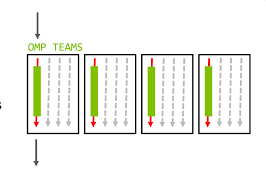
\includegraphics[width=0.75\textwidth]{target_teams}
\centering
\captionsetup{justification=centering, singlelinecheck=false}
	\caption{Ομάδες νημάτων με την οδηγία \emph{\en{target teams \cite{target_teams}}}}
\label{fig:target_teams}
\end{figure}


\selectlanguage{english}
\begin{lstlisting}[language=C++, caption={\el{Φράσεις οδηγίας} \emph{\en{target}} } , frame=tlrb]{Name}
num_teams (integer-expression)
threadJimit (integer-expression)
default(shared I none)
private (list)
firstprivate (list)
shared (list)
reduction (reduction-identifier : list)
\end{lstlisting}
\selectlanguage{greek}

\subsubsection{Η οδηγία \en{distribute}}
\subparagraph{}


\selectlanguage{english}
\begin{lstlisting}[language=C++, caption={\el{Σύνταξη οδηγίας} \emph{\en{distribute}} } , frame=tlrb]{Name}
#pragma omp distribute {clause[[,} clause}. . . j
	for-loops
\end{lstlisting}
\selectlanguage{greek}


\selectlanguage{english}
\begin{lstlisting}[language=C++, caption={\el{Φράσεις υποστηριζόμενες από την οδηγία} \emph{\en{distribute}} } , frame=tlrb]{Name}
private {list)
firstprivate {list)
lastprivate {list)
collapse (n)
dist_schedule {kind[, chunk_sizej)
\end{lstlisting}
\selectlanguage{greek}

Η οδηγία  \emph{\en{distribute}} καθορίζει τον διαμοιρασμό  επαναλήψεων ενός βρόγχου στα αρχικά νήματα των ομάδων που δημιουργήθηκαν από την οδηγία \emph{\en{target teams}}. Οι επαναλήψεις του βρόγχου χωρίζονται σε τμήματα και μοιράζονται στα κύρια νήματα των ομάδων. Η οδηγία \emph{\en{distribute}} δεν εχει υπονοούμενο φράγμα εργασιών στο τέλος της, πράγμα που σημαίνει οτι τα κύρια νήματα των ομάδων δε συγχρονίζονται στο τέλος της οδηγίας.

Η φράση \emph{\en{distschedule}} καθορίζει τον τρόπο που διαμοιράζονται οι επαναλήψεις σε τμήματα. Συγκριτικά με την οδηγία \emph{\en{for}} η \emph{\en{distribute}} έχει δυνατότητες για καλύτερη απόδοση. Ο μεταγλωττιστής μπορεί να πετύχει μεγαλύτερη βελτιστοποίηση.



\subsubsection{Σύνθετες οδηγίες επιταχυντών}
\subparagraph{}

Οι συνδυασμένες οδηγίες είναι ισοδύναμες με τις επιμέρους. Για παράδειγμα η οδηγία \emph{\en{parallel for}} έχει την ιδια σημασία με την \emph{\en{parallel}} ακολουθούμενη από την οδηγία \emph{\en{for}}. Παρόλα αυτά, ορισμένες φορές, οι συνδυασμένες οδηγίες μπορούν να επιτύχουν καλύτερες επιδόσεις.
Σε αυτή την παράγραφο, οι οδηγίες χωρίζονται σε δύο κατηγορίες, τις συνδυασμένες με \emph{\en{target}} και αυτές που συνδυάζονται με \emph{\en{target teams}}.

\selectlanguage{english}
\begin{lstlisting}[language=C++, caption={\el{Συνδυασμένες οδηγίας επιταχυντή}} , frame=tlrb]{Name}
#pragma omp target parallel [clause[[,] clause]...]
	structured block

#pragma omp target parallel for [clause[[,] clause]...]
	for-loops
	
#pragma omp target parallel for simd [clause[[,] clause]...]
	for-loops
	
#pragma omp target simd [clause[[,] clause]...]
	for-loops
\end{lstlisting}
\selectlanguage{greek}


\selectlanguage{english}
\begin{lstlisting}[language=C++, caption={\el{Συνδυασμένες οδηγίας επιταχυντή}} , frame=tlrb]{Name}
#pragma omp distribute parallel for [clause[[,] clause]...]
	for-loops
#pragma omp distribute simd [clause[[,] clause]...]
	for-loops
#pragma omp distribute parallel for simd [clause[[,] clause]...]
	for-loops
\end{lstlisting}
\selectlanguage{greek}


\subsubsection{Φράσεις οδηγίας \emph{\en{map}}}
\subparagraph{}
\selectlanguage{english}
\begin{lstlisting}[language=C++, caption={\el{Σύνταξη οδηγίας} map} , frame=tlrb]{Name}
map ([[map-type-modifier[,}} map-type:} list)

\end{lstlisting}
\selectlanguage{greek}
\selectlanguage{english}
\begin{lstlisting}[language=C++, caption={\el{Αποδεκτές τιμές για το } map-type} , frame=tlrb]{Name}
	alloc
	to
	from
	tofrom -> default
	release
	delete
\end{lstlisting}
\selectlanguage{greek}

Υπάρχουν τρεις φάσεις στην αντιστοίχιση μεταβλητών στον επιταχυντή:
\begin{enumerate}
  \item Η φάση \emph{\en{map-enter}} στην αρχή της εκτέλεσης της οδηγίας \emph{\en{target}}, όπου οι μεταβλητή αντιστοιχίζεται στον επιταχυντή. Σε αυτή τη φάση δεσμεύεται μνήμη του επιταχυντή για την αποθήκευση της μεταβλητής, και αντιγράφεται από τον εξυπηρετητή.
  \item Η φάση υπολογισμού που προκύπτει όταν, κατά τη διάρκεια εκτέλεσης της παράλληλης περιοχής, τα νήματα που εκτελούν το πρόγραμμα αποκτούν πρόσβαση στην αντιστοιχισμένη μεταβλητή.
  \item Η φάση εξόδου όπου ολοκληρώνεται η αντιστοίχιση των μεταβλητών στον επιταχυντή. Η τιμή της μεταβλητής στον επιταχυντή αντιγράφεται στην αντίστοιχη θέση του εξυπηρετητή. Η δεσμευμένη μνήμη του επιταχυντή ελευθερώνεται.
\end{enumerate}

Οι φάσεις 1 και 3 διαχειρίζονται την αποθήκευση και αντιγραφή των μεταβλητών ανάμεσα σε δυο συσκευές. Ο τύπος της αντιστοίχισης επηρεάζει την αντιγραφή μεταβλητών στον επιταχυντή ή τον εξυπηρετητή. Ο καθορισμός του τύπου αντιστοίχισης επηρεάζει την απόδοση του κώδικα.


\begin{table}[htbp]
\captionsetup{justification=raggedright,
singlelinecheck=false
}
\caption{Απαιτούμενη αντιγραφή για κάθε τύπο μεταβλητής κατά τις φάσεις εισόδου-εξόδου}
\def\arraystretch{1.5}
\begin{tabular}{| p{0.25\textwidth} | p{0.25\textwidth}|  p{0.25\textwidth} |  p{0.25\textwidth}|}
 \en{map-type}\cellcolor[HTML]{D0D0D0} & \textbf{Είσοδος} \cellcolor[HTML]{D0D0D0} & \textbf{Έξοδος}\cellcolor[HTML]{D0D0D0} \\
\hline
\textbf{\en{alloc}} & Οχι & Οχι \\
\hline
\textbf{\en{to}} & Ναι & Οχι \\
\hline
\textbf{\en{from}} & Οχι & Ναι \\
\hline
\textbf{\en{tofrom}} & Ναι & Ναι \\
\hline
\textbf{\en{release}} & - & Οχι \\
\hline
\textbf{\en{delete}} & - & Οχι \\
\hline
\end{tabular}
\end{table}

\clearpage
\selectlanguage{english}
\begin{lstlisting}[language=C++, caption={\el{Παράδειγμα χρήσης τύπου αντιστοίχισης μεταβλητών}} , frame=tlrb]{Name}
void foo(double A[1024], double B[1024], double C[1024) {
	#pragma omp target map(from : A) map(to: B) 
			map(alloc: C) // map enter
	{
		//CODE
	} // map exit
}
\end{lstlisting}
\selectlanguage{greek}

Στο προηγούμενο παράδειγμα:

Η μεταβλητή \textbf{Α}:
\begin{itemize}
  \item Δεν αρχικοποιείται στον επιταχυντή
  \item Οι τιμή της αντιγράφεται στον εξυπηρετητή
  \item Η μνήμη αποδεσμεύεται κατά την επιστροφή στον εξυπηρετητή.
\end{itemize}
\ \\
Η μεταβλητή \textbf{Β}:
\begin{itemize}
  \item Οι τιμή της αντιγράφεται στον επιταχυντή.
  \item Η μνήμη αποδεσμεύεται κατά την επιστροφή στον εξυπηρετητή.
\end{itemize}
\ \\
Η μεταβλητή \textbf{\en{C}}:
\begin{itemize}
  \item Οι τιμή της αντιγράφεται στον επιταχυντή.
  \item Η μνήμη αποδεσμεύεται κατά την επιστροφή στον εξυπηρετητή.
\end{itemize}

\subsubsection{Οδηγία \emph{\en{declare target}}}
\subparagraph{}
Η οδηγία \emph{\en{declare target}} χρησιμοποιείται για συναρτήσεις και μεταβλητής. Μια συνάρτηση που καλείται μέσα στο τμήμα του \emph{\en{target}} κώδικα, θα πρέπει να δηλώνεται στην οδηγία \emph{\en{declare target}}. Ακόμη, η οδηγία χρησιμοποιείται για την αντιστοίχιση \emph{\en{global}} μεταβλητών στο περιβάλλον δεδομένων του επιταχυντή.



\selectlanguage{english}
\begin{lstlisting}[language=C++, caption={\el{Συνδυασμένες οδηγίας επιταχυντή}} , frame=tlrb]{Name}
#pragma omp declare target
	declarations-definitions-seq
#pragma omp end declare target
#pragma omp declare target(extended-list)
#pragma omp declare target clause[[l] clause]...]

CLAUSE:
to (extended-list)
link (list)
\end{lstlisting}
\selectlanguage{greek}

\textbf{\en{TODO}} έχει και αλλο.
